\chapter{Lec 15 - Sequence Modeling}

\section{Learning in Sequential Domains}
Why learning in sequential domains is different than static domains ? Because successive points in sequential data are \textbf{strongly correlated}. Machine learning models and algorithms for sequence learning have to consider that data points are not independent, deal with sequential distortions and/or variations (e.g. In speech, variations in speaking rate) and make use of \textbf{contextual information}.
\newline\newline
With static data we usually learn:
\[P(\textbf{o}|\textbf{x})\]
where $\textbf{x}$ is a fixed-size tuple of predictive attributes and $\textbf{o}$ is a classification/regression task.\newline\newline
With \textbf{sequential data}, instead, $\textbf{x}$ is a \textbf{sequence} $x^{(1)}, ..., x^{(t)}, ...$ where each $x^{(t)}$ has a static type. $\textbf{o}$ may be either static (e.g., sequence classification) or a sequence.\newline\newline
Using mathematical induction, a \textbf{sequence} is either an external vertex, or an ordered pair $(t, h)$ where the head $h$ is a vertex and the tail $t$ is a sequence.

\subsection{Sequencial Transductions}
Sequence Transduction is a machine learning task that involves converting an input sequence into an output sequence, potentially of different lengths.\newline\newline
Let $X$ and $O$ be the \textbf{input} and \textbf{output} label spaces. We denote by $X^*$ the set of all sequences with labels in $X$. We can define a general transduction $T$ as a function
\[T : X^* \rightarrow O^*\]
\begin{itemize}
    \item $T(\cdot)$ has \textbf{finite memory} $k \in \mathbb{N}$ if $\forall \textbf{x} \in X^*$ and $\forall t$, $T(x^{(t)})$ only depends on $\{\textbf{x}^{(t)}, \textbf{x}^{(t-1)}, ..., \textbf{x}^{(t-k)}\}$ 

    \item $T(\cdot)$ is \textbf{algebraic} if it has 0 finite memory (i.e., no memory at all)

    \item A transduction $T(\cdot)$ is \textbf{causal} if the output at time $t$ does not depend on future inputs (at time $t + 1, t + 2,...$ )

\end{itemize}

\subsection{Learning Sequences}
Sequences have variable length but typical machine learning models
have a fixed number of inputs. In order to solve this problem we can:
\begin{itemize}
    \item Limit context to a \textbf{fixed-size window}.
    \item Use \textbf{recurrent} models.
    \item Use \textbf{transformers} for non-causal sequences (e.g. text).
\end{itemize}


\section{Recursive State Representation}
In order to represent a recursive state we can use the following equations:
\[\begin{split}
    h^{(t)} & = f(h^{(t-1)}, x^{(t)}, t)\\
    o^{(t)} & = g(h^{(t)}, x^{(t)}, t)
\end{split}\]
where $f$ is the \textit{state transition function} and $g$ is the \textit{output function}. 
\newline\newline
$h^{(t)}$ is called the state of the system and it's defined by a \textbf{recursive equation}. Indeed, the definition of $h$ at time $t$ refers back to the same definition at time $t - 1$. It contains information about the whole past sequence. For a finite number of time steps $\tau$, the graph can be unfolded by applying the definition $\tau - 1$ times. \textbf{Unfolding} the equation by repeatedly applying the definition yields an expression that does not involve recurrence. Such an expression can now be represented by a traditional directed acyclic computational graph.
\begin{center}
    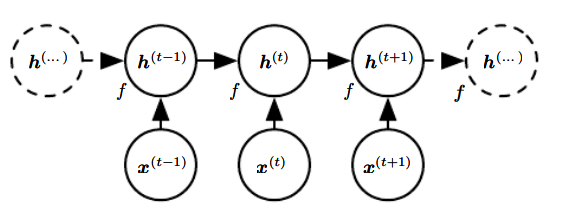
\includegraphics[]{images/recurrent-graph.png}
\end{center}
The state transition function can be represented using the time shift operator $q^{-1}$:
\[q^{-1}h^{(t)} = h^{(t-1)}\]
\begin{center}
    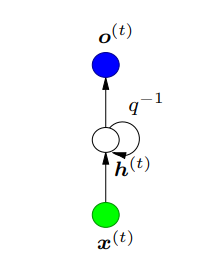
\includegraphics[]{images/time-shift-op.png}
\end{center}
The unfolding process thus introduces two major advantages:
\begin{enumerate}
    \item Regardless of the sequence length, the learned model always has the same input size, because it is specified in terms of transition from one state to another state, rather than specified in terms of a variable-length history of states.

    \item It is possible to use the same transition function $f$ with the same parameters at every time step.
\end{enumerate}
These two factors make it possible to learn a single model that operates on all time steps and all sequence lengths. Learning a single, shared model allows generalization to sequence lengths that did not appear in the training set, and allows the model to be estimated with far fewer training examples than would be required without parameter sharing.\newline\newline
Given a sequence $s \in X^{*}$ and a recursive transduction $T$, the \textit{encoding network} associated to $s$ and $T$ is formed by unrolling (time unfolding) the recursive network of $T$ through the input sequence $s$.
\begin{center}
    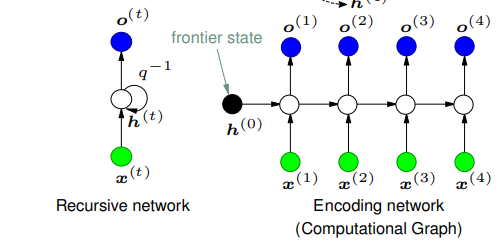
\includegraphics[]{images/encoding-network.png}
    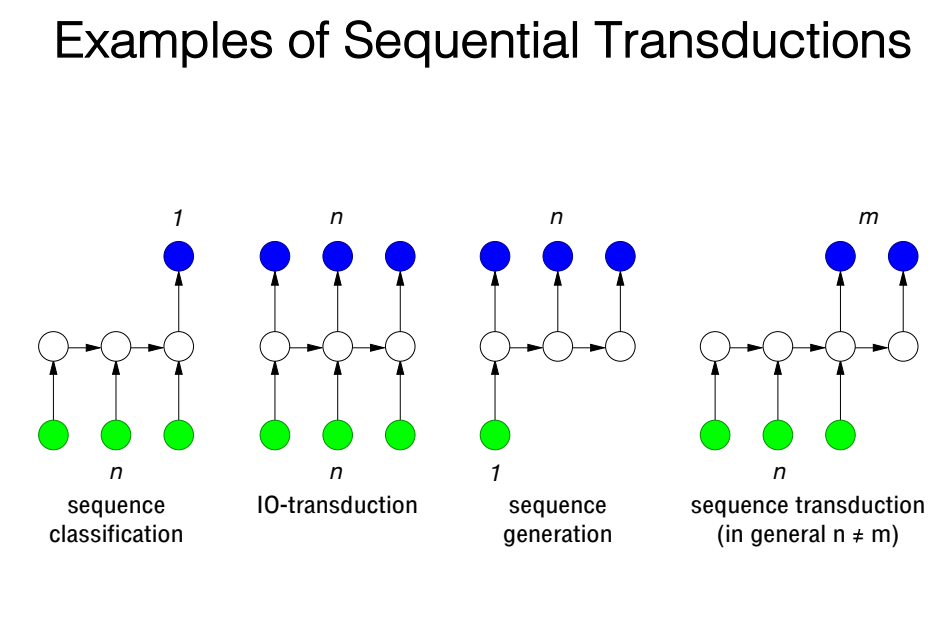
\includegraphics[scale=0.7]{images/sequential--transduction.png}
\end{center}
$T$ is \textbf{stationary} if $f(\cdot)$ and $g(\cdot)$ do not depend on $t$\newline\newline
There are different ways in which we can implement $f(\cdot)$ and $g(\cdot)$. There are two general families of models:
\begin{itemize}
    \item Linear:
    \begin{itemize}
        \item Kalman Filter
        \item Hidden Markov Models
        \item Linear Dynamical Systems
        \item ...
    \end{itemize}
    \item Nonlinear
    \begin{itemize}
        \item Recurrent Neural Networks
        \item ...
    \end{itemize}
\end{itemize}

\section{Shallow Recurrent Neural Networks}
Armed with the graph unrolling and parameter sharing ideas, we can design a wide variety of recurrent neural networks. In general we have:
\[\begin{split}
    \textbf{h}^{(t)} & = f(\textbf{U}\textbf{x}^{(t)} + \textbf{W}\textbf{h}^{(t-1)} + \textbf{b})\\
    \textbf{o}^{(t)} & = g(\textbf{V}\textbf{h}^{(t)} + \textbf{c})
\end{split}\]
where $f()$ and $g()$ are non-linear functions (e.g. $tanh()$ and $softmax$), and $h^{(0)} = 0$ (or can be learned jointly with the other parameters). $\textbf{U}$ and $\textbf{W}$ are weight matrices which parametrize \textbf{input-to-hidden} connections and \textbf{hidden-to-hidden} recurrent connections respectively. \textbf{Hidden-to-output} connections are parametrized by the weight matrix $\textbf{V}$.\newline\newline
An example of RNN for IO-transduction with discrete outputs:
\[\begin{split}
    \textbf{h}^{(t)} & = tanh(\textbf{U}\textbf{x}^{(t)} + \textbf{W}\textbf{h}^{(t-1)} + \textbf{b})\\
    \textbf{o}^{(t)} & = \textbf{V}\textbf{h}^{(t)} + \textbf{c}\\
    \hat{\textbf{y}} & = softmax(\textbf{o}^{(t)})\\
    L & = \sum_t L^{(t)} = - \sum_t log\,p_{model}(\textbf{y}^{(t)} | \{\textbf{x}^{1}, ..., \textbf{x}^{(t)}\})
\end{split}\]
where:
\begin{itemize}
    \item $o^{(t)}$ is the unnormalized log probabilities a time $t$
    \item $\textbf{y}^{(t)}$ is the target vector a time $t$
    \item $p_{model}(\textbf{y}^{(t)} | \{\textbf{x}^{1}, ..., \textbf{x}^{(t)}\}$ is given by reading the entry for $\textbf{y}^{(t)}$ from the model’s output vector $\hat{\textbf{y}}^{(t)}$, that is, the loss $L$ \textbf{internally computes} $\hat{\textbf{y}}$.
    \item $L$ is the loss function
\end{itemize}
The corresponding computation graph is the following
\begin{center}
    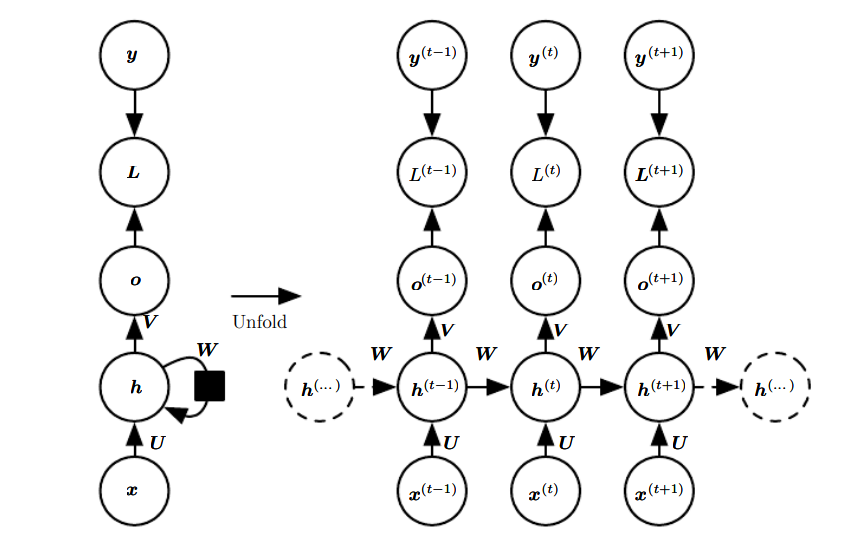
\includegraphics[scale=0.8]{images/rnn-computational-graph.png}
\end{center}
Some examples of important design patterns for recurrent neural networks
include the following:
\begin{itemize}
    \item Recurrent networks that produce an output at each time step and have recurrent connections between hidden units (IO-transduction).

    \item Recurrent networks that produce an output at each time step and have recurrent connections only from the output at one time step to the hidden units at the next time step

    \item Recurrent networks with recurrent connections between hidden units, that read an entire sequence and then produce a single output (e.g. for classification).
\end{itemize}
There are a lot of possible additional architectural features, such as short-cut connections, higher-order states, feedback from output, teacher forcing, bidirectional RNN, etc\footnote{See slides for further information}. All these architectural features (and others...) are orthogonal, i.e. they can be combined together.


\subsection{Teacher Forcing}
The network with recurrent connections only from the output at one time step to the hidden units at the next time step is strictly less powerful because it lacks hidden-to-hidden recurrent connections. Therefore, it requires that the output units capture all of the information about the past that the network will use to predict the future. Because the output units are explicitly trained to match the training set targets, they are unlikely to capture the necessary information about the past history of the input.\newline\newline
For this reason, models that have recurrent connections from their outputs leading back into the model may be trained with \textbf{teacher forcing}. Teacher forcing is a procedure in which during training the model receives the ground truth output $\textbf{y}^{(t)}$ as input at time $t + 1$. When the model is deployed, the true output is generally not known. In this case, we approximate the correct output $\textbf{y}^{(t)}$ with the model’s output $\textbf{o}^{(t)}$, and feed the output back into the model.
\[\begin{split}
    \textbf{h}^{(t)} & = tanh(\textbf{U}\textbf{x}^{(t)} + \textbf{W}\textbf{y}^{(t-1)} + \textbf{b})\\
    \textbf{o}^{(t)} & = \textbf{V}\textbf{h}^{(t)} + \textbf{c}\\
    \hat{\textbf{y}} & = softmax(\textbf{o}^{(t)})\\
    L & = - \sum_t log\,p_{model}(\textbf{y}^{(t)} | \textbf{y}^{(1)}, ..., \textbf{y}^{(t-1)}, \textbf{x}^{(1)}, ..., \textbf{x}^{(t)})
\end{split}\]
\begin{center}
    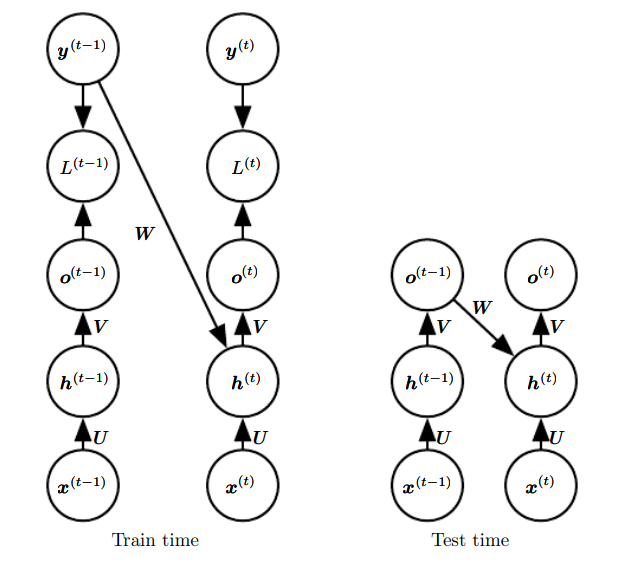
\includegraphics[]{images/teacher-forcing.png}
\end{center}
The advantage of eliminating hidden-to-hidden recurrence is that, for any loss function based on comparing the prediction at time $t$ to the training target at time $t$, all the time steps are decoupled. Training can thus be parallelized, with the gradient for each step $t$ computed in isolation.

\subsection{Bidirectional RNNs}
in many applications we want to output a prediction of $\textbf{y}^{(t)}$ which may depend on the whole input sequence. For example, if there
are two interpretations of the current word that are both plausible, we may have to look far into the future (and the past) to disambiguate them. Bidirectional recurrent neural networks (or bidirectional RNNs) were invented to address that need.\newline\newline
As the name suggests, bidirectional RNNs combine an RNN that moves forward
through time, beginning from the start of the sequence, with another RNN that moves backward through time, beginning from the end of the sequence.
\begin{center}
    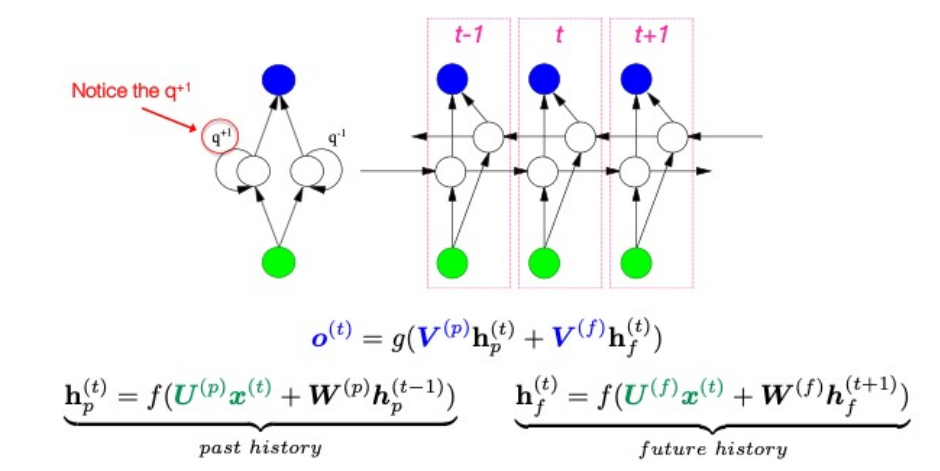
\includegraphics[scale=0.9]{images/bidirectional-rnn.png}
\end{center}

\subsection{1 to \textit{n} transduction}
Previously, we have discussed RNNs that take a sequence of vectors $\textbf{x}^{(t)}$ for $t = 1, ..., \tau$ as input. Another option is to take only a single vector $\textbf{x}$ as input. When $\textbf{x}$ is a fixed-size vector, we can simply make it an extra input of the RNN
that generates the $\textbf{y}$ sequence.  The interaction between the input $\textbf{x}$ and each hidden unit vector $\textbf{h}^{(t)}$ is parametrized by a newly introduced weight matrix $\textbf{R}$.
\begin{center}
    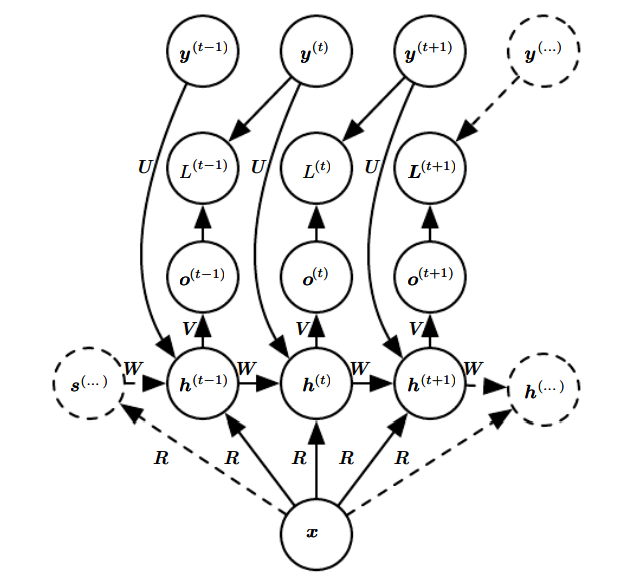
\includegraphics[scale=0.8]{images/1-to-n transduction.png}
\end{center}
Each element $\textbf{y}^{(t)}$ of the observed output sequence serves both as input (for the current hidden unit at time $t$) and, during training, as target (for the previous output unit at time $t-1$).\newline\newline
This RNN is appropriate for tasks such as image captioning, where a single image is used as input to a model that then produces a sequence of words describing the image.

\subsection{Encoder-Decoder Sequence-to-Sequence Architectures}
Here we discuss how an RNN can be trained to map an input sequence to an output sequence which is not necessarily of the same length. This comes up in many applications, such as speech recognition, machine translation, etc.\newline\newline
An encoder-decoder RNN architecture is is composed of an encoder RNN that reads the input sequence and a decoder RNN that generates the output sequence. The final hidden state of the encoder RNN is used to compute a generally fixed-size context variable $C$ which represents a semantic summary of the input sequence and is given as input to the decoder RNN.
\begin{center}
    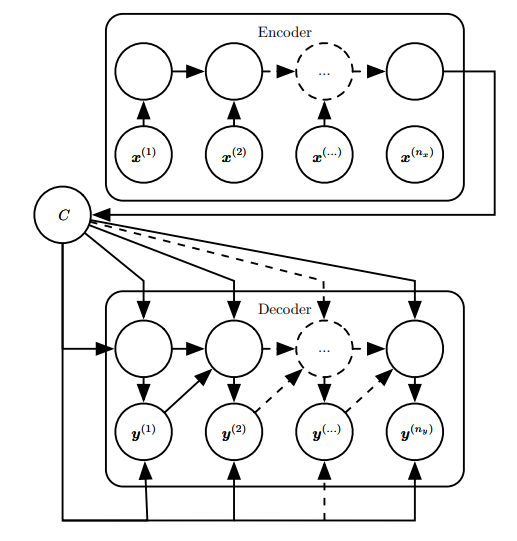
\includegraphics[]{images/encoder-decoder rnn.png}
\end{center}
If the context $C$ is a vector, then the decoder RNN is simply a vector-to-sequence RNN.

